\documentclass{beamer} % [mathserif]
\usepackage{amsmath}
\usepackage{graphicx}
\usepackage{subfigure}
\usepackage{wrapfig}
\usepackage{booktabs}
\usepackage{hyperref}
\usepackage{media9}
% \usepackage{pgfplots}
% \pgfplotsset{compat=1.18}
% \usepgfplotslibrary{dateplot}
% \usepackage{tipa}
% \usepackage{epstopdf} % this is needed for windows Texworks
\usepackage[absolute,overlay]{textpos} % ,showboxes

\setlength{\TPHorizModule}{1in}
\TPVertModule=\TPHorizModule

\DeclareGraphicsExtensions{.eps}

\usetheme{Marburg}
% \usetheme{Berkeley}
% \usecolortheme{rose}
\definecolor{naublue}{HTML}{002454}
\definecolor{nauyellow}{HTML}{FAC01A}
%\setbeamercolor{structure}{bg=nauyellow, fg=naublue}
\setbeamercolor{palette primary}{bg=nauyellow, fg=naublue}
\setbeamercolor{palette secondary}{bg=nauyellow, fg=naublue}
%%%% See https://en.wikibooks.org/wiki/LaTeX/Presentations#User-defined_themes
% \setbeamercolor{alerted text}{fg=orange}
% \setbeamercolor{background canvas}{bg=white}
% \setbeamercolor{block body alerted}{bg=normal text.bg!90!black}
% \setbeamercolor{block body}{bg=normal text.bg!90!black}
% \setbeamercolor{block body example}{bg=normal text.bg!90!black}
% \setbeamercolor{block title alerted}{use={normal text,alerted text},fg=alerted text.fg!75!normal text.fg,bg=normal text.bg!75!black}
% \setbeamercolor{block title}{bg=blue}
% \setbeamercolor{block title example}{use={normal text,example text},fg=example text.fg!75!normal text.fg,bg=normal text.bg!75!black}
% \setbeamercolor{fine separation line}{}
\setbeamercolor{frametitle}{fg=naublue}
% \setbeamercolor{item projected}{fg=black}
% \setbeamercolor{normal text}{bg=black,fg=yellow}
% \setbeamercolor{palette sidebar primary}{use=normal text,fg=normal text.fg}
\setbeamercolor{palette sidebar primary}{bg=naublue, fg=nauyellow}
% \setbeamercolor{palette sidebar quaternary}{use=structure,fg=structure.fg}
% \setbeamercolor{palette sidebar secondary}{use=structure,fg=structure.fg}
% \setbeamercolor{palette sidebar tertiary}{use=normal text,fg=normal text.fg}
\setbeamercolor{section in sidebar}{fg=nauyellow, bg=naublue}
\setbeamercolor{section in sidebar shaded}{fg=white}
% \setbeamercolor{separation line}{}
% \setbeamercolor{sidebar}{bg=red}
% \setbeamercolor{sidebar}{parent=palette primary}
% \setbeamercolor{structure}{bg=black, fg=green}
% \setbeamercolor{subsection in sidebar}{fg=brown}
% \setbeamercolor{subsection in sidebar shaded}{fg=grey}
\setbeamercolor{title}{fg=naublue}
% \setbeamercolor{titlelike}{fg=brown}

% \usepackage[latin1]{inputenc}

%%%% See https://en.wikibooks.org/wiki/LaTeX/Presentations#Title_page_and_author_information
\title[INF632 (EE499/EE599)]{Wearable Technologies and Applications\\(Wearable Informatics)} %
\author{Winfree}
\date{Lecture 4}
%\institute{Northern Arizona University}

%\logo{\includegraphics[width=.5in]{figures/logo}}
% \setbeameroption{show notes on second screen}

\begin{document}
	\maketitle


\section[Outline]{}
\frame{\tableofcontents}

% \begin{frame}
%   \frametitle{Image Example}
%   \includegraphics[width=0.8\linewidth]{figures/_seikowrist.jpg}
% \end{frame}

\section{Clinical Standards of Wearable Devices (PA)}
	\subsection{Devices}
	\begin{frame}
		\frametitle{Devices}
		\centering
		%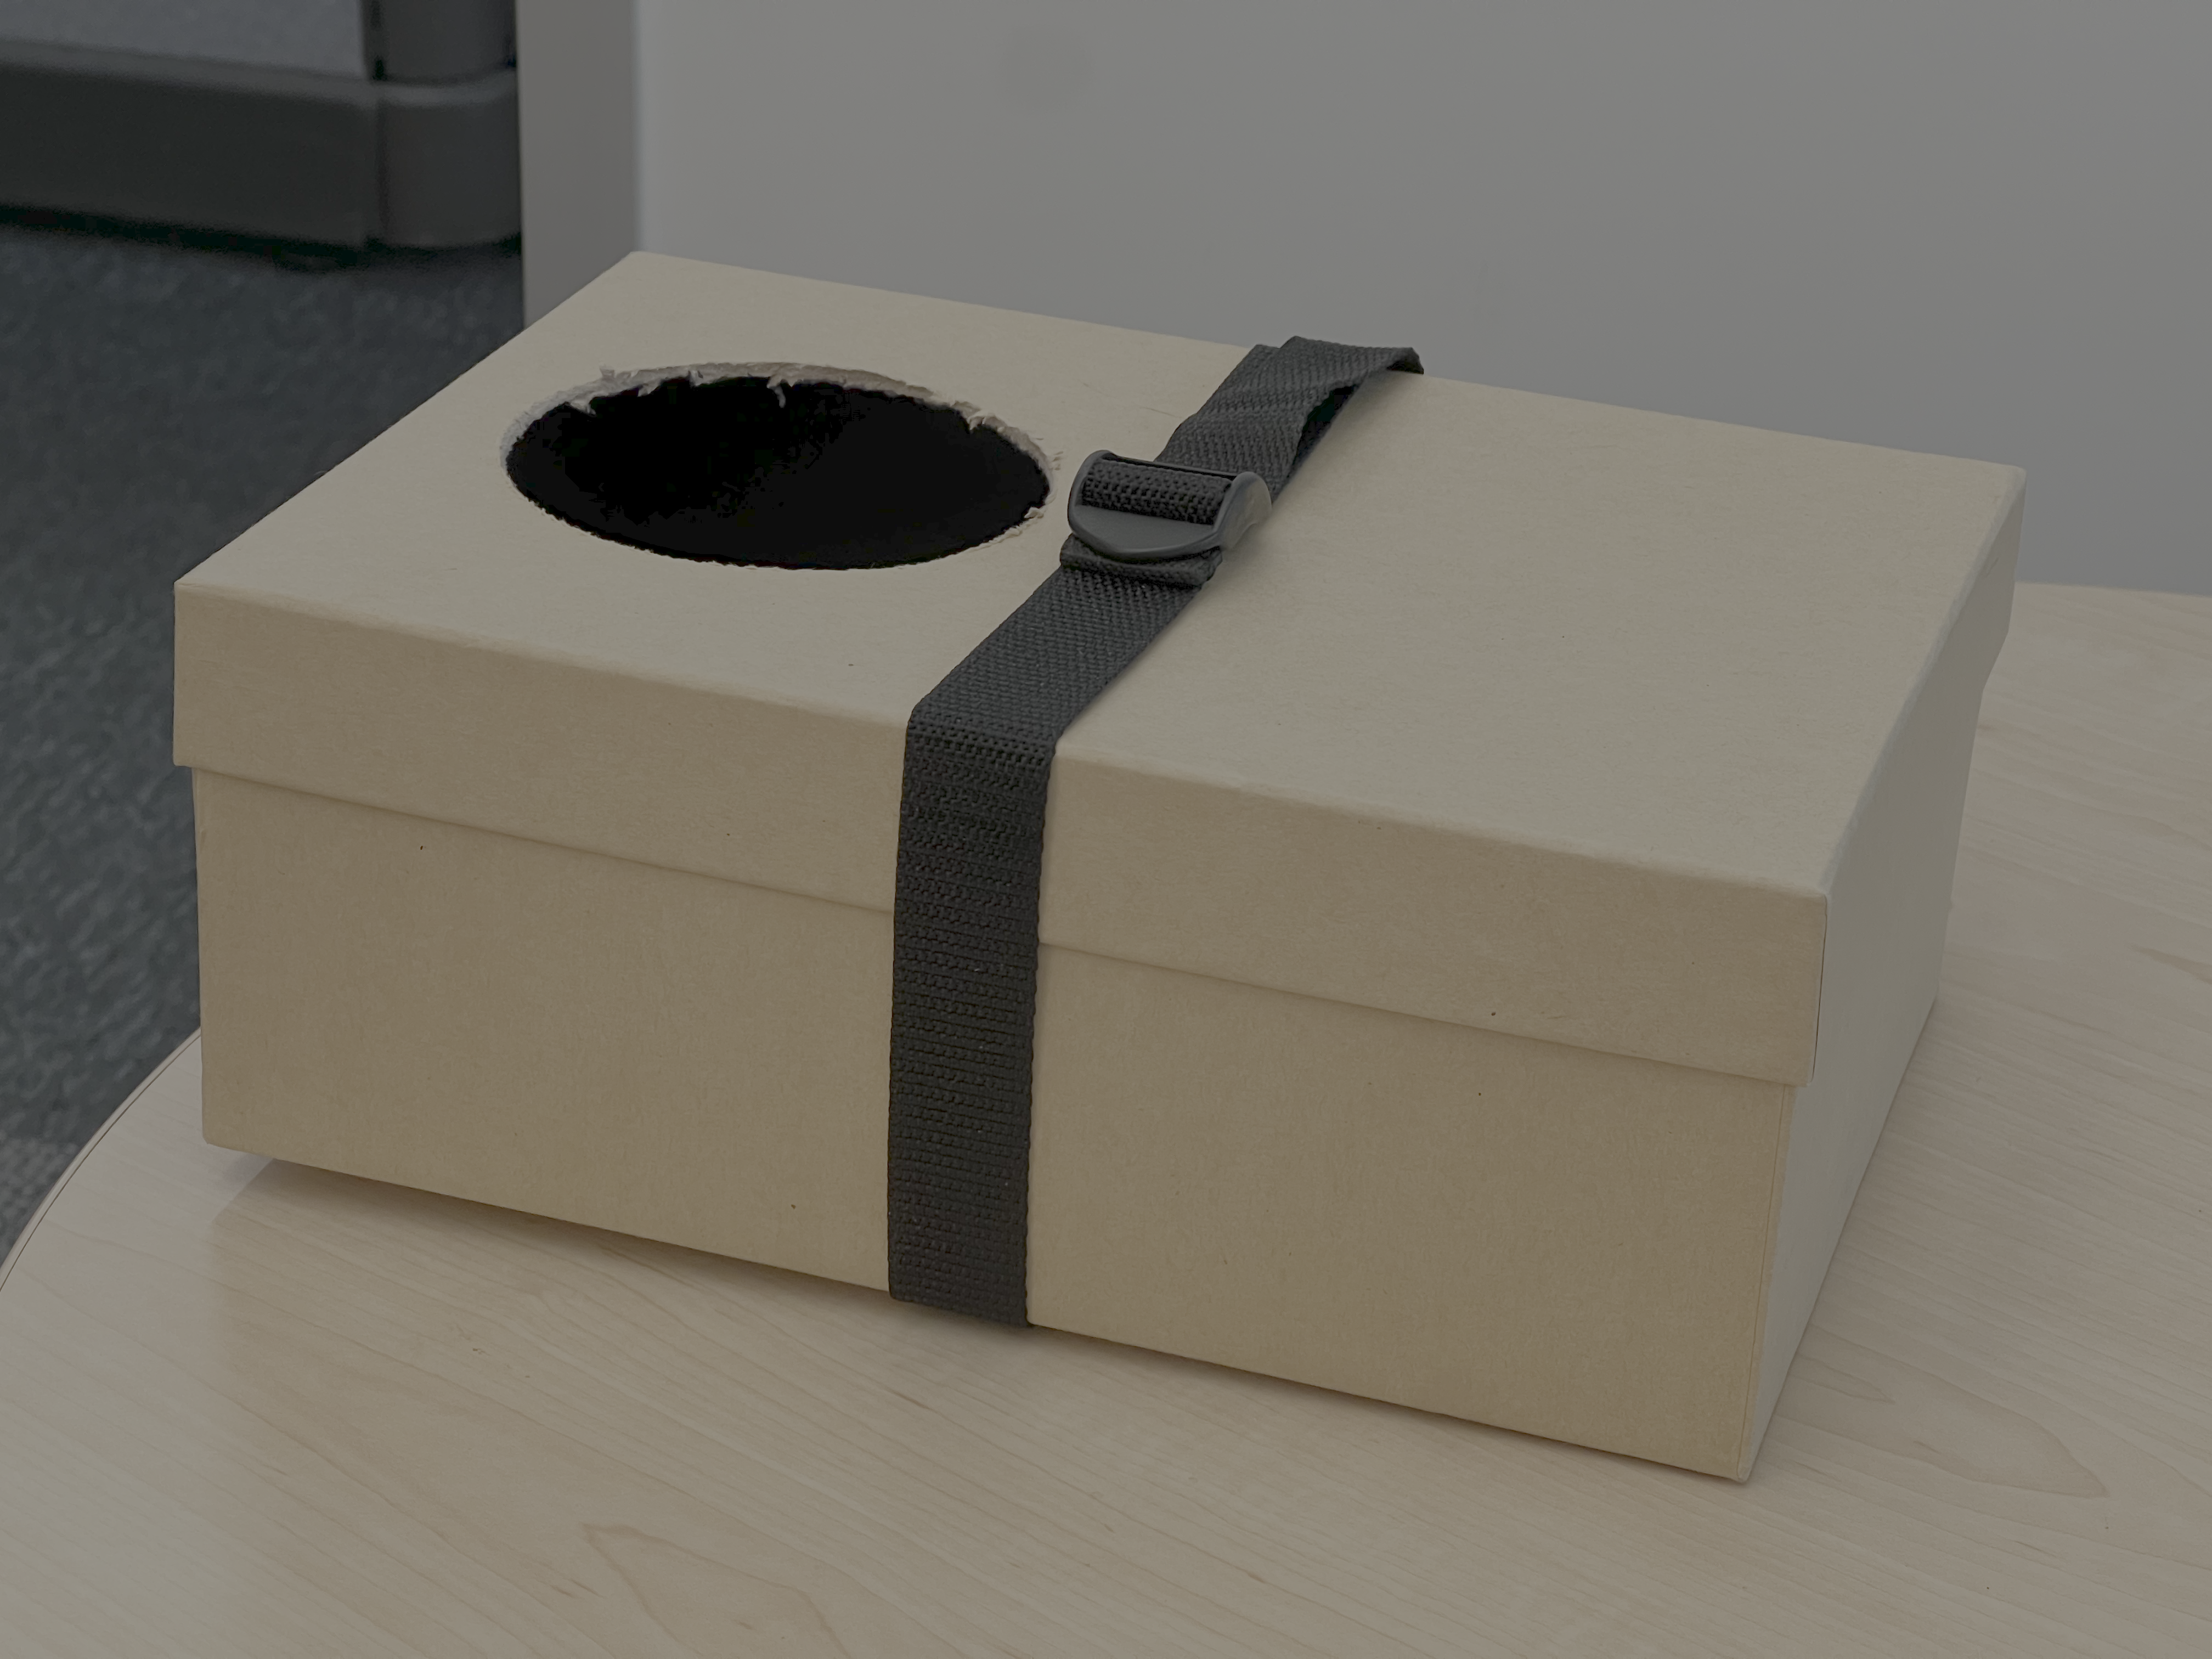
\includegraphics[width=1\linewidth]{figures/IMG_3915.png}
	\end{frame}
	
	\subsection{Data Transfer}
	\begin{frame}
		\frametitle{Data Transfer}
		\begin{columns}
			\begin{column}{.25\linewidth}
				\begin{itemize}
					\item Hearing?
					\item Sight?
					\item Smell?
					\item Taste?
					\item Touch?
				\end{itemize}
			\end{column}
			\begin{column}{.25\linewidth}
				%\includegraphics[width=1\linewidth]{figures/4 stick figure high point phase of walk cycle animation tutorial the helpful art teacher.JPG}
			\end{column}
			\begin{column}{.5\linewidth}
				\begin{itemize}
					\item Which of these seems the most valuable to you?
					\item Which would you relinquish last?
				\end{itemize}
			\end{column}
		\end{columns}
	\end{frame}
	
	\subsection{Data}
	\begin{frame}
		\frametitle{Data}
		\begin{columns}
			\begin{column}{.375\linewidth}
				Sight
				%\includegraphics[width=1\linewidth]{figures/intoxicating_eye_stock_by_taylorinchains-d35yf9n.jpg}
				\begin{itemize}
					\item Centralized
					\item Broad
					\item Passive
					\item Cognitive
				\end{itemize}
			\end{column}
			\begin{column}{.25\linewidth}
				%\includegraphics[width=1\linewidth]{figures/4 stick figure high point phase of walk cycle animation tutorial the helpful art teacher.JPG}
			\end{column}
			\begin{column}{.375\linewidth}
				~ % empty, so that it all appears on the next slide
			\end{column}
		\end{columns}
	\end{frame}
	
	\subsection{Typical Analysis}
	\begin{frame}
		\frametitle{Typical Analysis}
		\begin{columns}
			\begin{column}{.375\linewidth}
				\begin{center}
					Sight
				\end{center}
				%\includegraphics[width=1\linewidth]{figures/intoxicating_eye_stock_by_taylorinchains-d35yf9n.jpg}
				\begin{itemize}
					\item Centralized
					\item Broad
					\item Passive
					\item Cognitive
				\end{itemize}
			\end{column}
			\begin{column}{.25\linewidth}
				%\includegraphics[width=1\linewidth]{figures/4 stick figure high point phase of walk cycle animation tutorial the helpful art teacher.JPG}
			\end{column}
			\begin{column}{.375\linewidth}
				\begin{center}
					Touch
				\end{center}
				%\includegraphics[width=1\linewidth]{figures/wrist-drop.jpg}
				\begin{itemize}
					\item Distributed
					\item Narrow
					\item Interactive
					\item Fundamental
				\end{itemize}
			\end{column}
		\end{columns}
	\end{frame}

\section{Analysis}
	\subsection{Central Tendency}
	\begin{frame}
		\frametitle{Central Tendency}
	  %\setbeamercovered{transparent=20}
		\begin{definition}
			haptic\\ %\textcolor{gray}{| \textipa{/ˈwɛərəbl/} |}\\ % or 'wer\schwa b(\schwa)l 
			\textbf{adjective}\\
			\begin{enumerate}
				\item of or relating to the sense of touch, in particular relating to the perception and manipulation of objects using the senses of touch and proprioception.
			\end{enumerate}
			\textbf{origin}\\
			\begin{enumerate}
				\item late 19th century: from Greek {\em haptikos} {\bf `able to touch or grasp,'} from {\em haptein} {\bf `fasten.'}
			\end{enumerate}
		\end{definition}
	\end{frame}
	
	\subsection{Measures of Variance}
	\begin{frame}
		\frametitle{Measures of Variance}
		\begin{definition}
			optics\\ %\textcolor{gray}{| \textipa{/ˌinfərˈmadiks/} |}\\
			\textbf{plural noun}\\
			\begin{enumerate}
				\item the \underline{scientific study of} sight and the behavior of light, or the properties of transmission and deflection of other forms of radiation.
			\end{enumerate}
		\end{definition}
		\begin{definition}
			in\textbullet for\textbullet mat\textbullet ics\\ %\textcolor{gray}{| \textipa{/ˌinfərˈmadiks/} |}\\
			\textbf{plural noun}\\
			\begin{enumerate}
				\item the \underline{science of} processing data for storage and retrieval; informatics science
			\end{enumerate}
		\end{definition}
	\end{frame}
	
	\subsection{Standardized Measures}
	\begin{frame}
		\frametitle{Standardized Measures (Z-Score)}
		\begin{definition}
		Haptics
			\begin{itemize}
				\item the science and technology of touch
			\end{itemize}
		\end{definition}
	\end{frame}
	
	\subsection{Comparison Tests}
	\begin{frame}
		\frametitle{Comparison Tests}
		pre post
		
		two groups
	\end{frame}
	
	\subsection{Analysis of Variance}
	\begin{frame}
		\frametitle{Anlaysis of Variance (ANOVA)}
		stuff
	\end{frame}

% \section{Readings}
% 	\subsection{Thursday}
% 		\begin{frame}
% 		\frametitle{Thrusday}
% 		\footnotesize
% 			\begin{itemize}
% 				\item OPTIONAL - Embodied Auxetic Intelligence in a Glove‐Type Wearable Haptic Interface Connecting Humans.pdf
% 				\item OPTIONAL - FiDTouch - A 3D Wearable Haptic Display for the Finger Pad.pdf
% 				\item OPTIONAL - Haptics in Teleoperated Medical Interventions -  Force Measurement, Haptic Interfaces and Their Influence on Users Performance.pdf
% 				\item OPTIONAL - Music Tactalizer - A Wearable Haptic Music Player with Multi-Feature Audio-Tactile Rendering.pdf
% 				\item OPTIONAL - Predicting the Future with Wearable Technology.pdf
% 				\item OPTIONAL - The Future of Wearable Technologies and Remote Monitoring in Health Care.pdf
% 				\item OPTIONAL - Ultralight Soft Wearable Haptic Interface with Shear‐Normal‐Vibration Feedback.pdf
% % 				\item {\em TO DISCUSS - Haptic Perception and Its Relation to Action.pdf}
% % 				\item {\em TO DISCUSS - Haptic Rendering Introductory Concepts.pdf}
% % 				\item {\em TO DISCUSS - The future of wearable technologies.pdf}
% 			\end{itemize}
% 		\end{frame}
% 		\begin{frame}
% 		\frametitle{Thrusday}
% 			\begin{itemize}
% 				\footnotesize
% 				\item OPTIONAL - Embodied Auxetic Intelligence in a Glove‐Type Wearable Haptic Interface Connecting Humans.pdf
% 				\item ...
% 				\item OPTIONAL - Ultralight Soft Wearable Haptic Interface with Shear‐Normal‐Vibration Feedback.pdf
% 				\normalsize
% 				\item {\bf TO DISCUSS - Haptic Perception and Its Relation to Action.pdf}
% 				\item {\bf TO DISCUSS - Haptic Rendering Introductory Concepts.pdf}
% 				\item {\bf TO DISCUSS - The future of wearable technologies.pdf}
% 			\end{itemize}
% 		\end{frame}
\end{document}
